\documentclass[titlepage, 12pt]{scrartcl}
\usepackage[utf8]{inputenc}
\usepackage{setspace}
\usepackage{subcaption}
\doublespacing
\usepackage[margin=1in]{geometry}
\usepackage{graphicx}
\usepackage[nottoc,numbib]{tocbibind}

%%% Maketitle metadata
\newcommand{\horrule}[1]{\rule{\linewidth}{#1}} 	% Horizontal rule
        
\title{
		\vspace{-1in} 	
		\usefont{OT1}{bch}{b}{n}
		\normalfont \normalsize \textsc{University of California, Los Angeles \\
		180DA Fall 2018 Final Report \\
		Professor Pottie} \\ [25pt]
		\horrule{0.5pt} \\
		\Huge ZombieArcher \\
		\vspace{-.3in}
		\horrule{2pt} \\
		\vspace{1in}
}

\author{Sidharth Bambah (904 787 435)\\
        Sparsh Gauba (204 600 605)\\
        Andrew Juarez (504 572 352)\\
        Mohamed Shatela (604 644 424)\\\\
        \vspace{1in}
        }

\date{ \large November 2018}

\begin{document}

\maketitle
\tableofcontents
\newpage
\section{Project Overview}
    The ZombieArcher project is an interactive augmented reality game which involves using a bow and arrow to fight zombie enemy AI. The purpose of the game beyond its entertainment aspect is to teach the user fundamental mechanics of how to aim and shoot an arrow to reach a target at various locations, and both static and moving targets. The game does so by providing the user with a controller that emulates the basic functions of a bow and arrow, namely the vertical and lateral angle of launch and the initial kinetic energy of the arrow, and by providing the user with a personalized training environment in which the user’s performance is measured in terms of accuracy, precision and reaction time. By collecting data regarding the user’s performance, the game adjusts the difficulty in each of the performance categories to help the user improve upon his or her weak points. \par
    The game design is inspired by first-person combat games, and as such, its graphical interface is a 3D world in which the player’s view is centered at the crosshair of the bow and arrow. From this viewpoint, the user knows only the initial launch direction of the arrow. The arrow, however, is subject to gravitational force, so depending on the distance of the target, the user has a range of correct combinations of launch angle and initial kinetic energy of the arrow to choose from. The game also provides the user with voice inputs and camera-based gestures to give additional inputs to the game such pausing and resuming the game, changing the type of arrow to launch, requesting additional zombies to spawn at specific locations on the map, and more. \par
    Looking beyond the scope of the game, the systems developed for this game can also be used in a wide range of other applications. The interactive wireless controller can be used as an input device for many other games and applications that require hand-eye coordination, as well as for teaching various types of physical tasks. Combined with the camera based gesture recognition, many simple medical applications are possible, such as physiotherapy, checking for abnormalities in posture, and more. Lastly, since the communication between the subsystems of the game is extensible, the game can also be extended for multiplayer and arcade games. \par

\section{Overall System}
    \begin{figure}
        \centering
        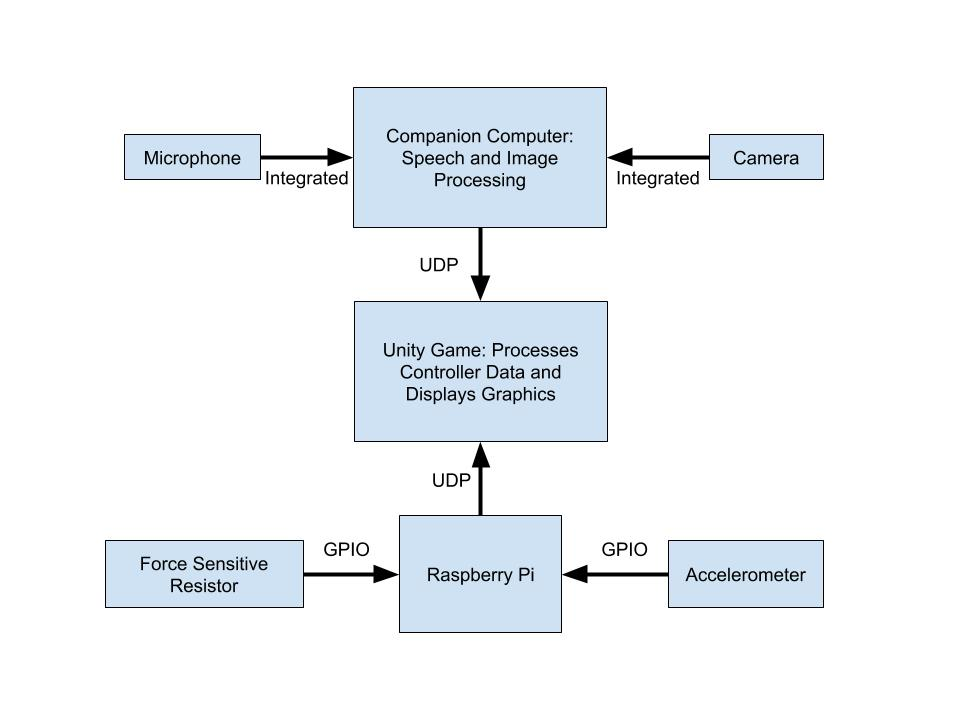
\includegraphics[scale=0.4]{figures/Block_Diagram.jpg}
        \caption{Block diagram of ZombieArcher with major subsystems and connections.}
        \label{fig:Block_Diagram}
    \end{figure}
    The diagram above shows the breakdown of the project into its subsystems. The host computer is tasked with receiving pre-processed data from the three user input systems to progress the next game state based on the inputs. The game logic and graphics are developed using Unity game engine. The physical controller is designed to physically resemble a bow with a bow string and a hand grip, and is powered by a Raspberry Pi Zero WH, which allows for wireless communication with the UDP server. The controller also houses the BerryIMU, which is integrates accelerometer, gyroscope, and magnetometer. This sensor enables measuring the controller's motion as the user aims at the target in game. The force sensor is used to measure the force by which the user pulls the bow string. A companion computer is used for interfacing with a microphone and web-cam and process the voice commands and gesture inputs using Google voice to text and OpenCV respectively. It then communicates the relevant game commands to the host computer via the UDP server. \par
    
\section{Hardware} 
    \subsection{Design}
    \begin{figure}
        \centering
        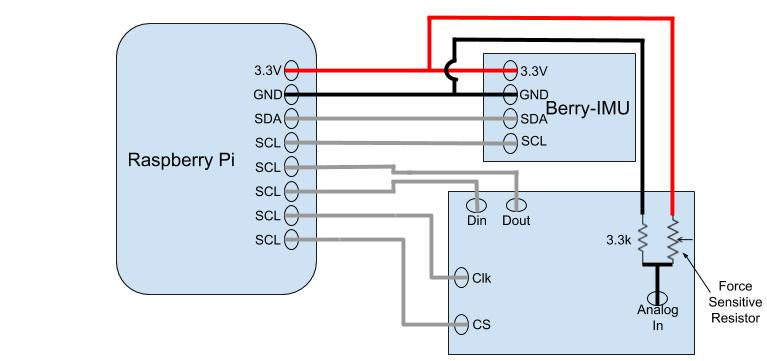
\includegraphics[scale=0.4]{figures/pi-pin.jpg}
        \caption{Wire connections between the major components of the controller.}
        \label{fig:pi-pin}
    \end{figure}
    The goal for the current physical iteration controller was to have a usable controller that was also easy to debug and modify. For initial testing of the electrical components, a breadboard was used. Initially, to measure the force the user is applying on the bow string, we had decided to use a strain gauge, which is a variable resistor whose resistance changes as the material it is attached to bends. This sensor was planned to be attached to a thin piece of metal that would be attached as a hand grip in the middle of the bow string. However, due to the high dependence on the physical properties of material to which it is attached, using this sensor would have limited the design of the controller's casing. Instead, the string pulling force is now measured by a force sensitive resistor, which more directly measures the amount of force being applied to its surface area. Due to the force sensitive resistor's fragile construction, it is now located under the hand grip for the bow's rigid portion rather than on the string. To convert the force sensitive resistor's value to digital, it is part of a voltage divider circuit, as shown in Figure 2. Increasing the force reduces the sensor's resistance, and the circuit is designed to measure the voltage across the constant resistor that is connected to the ground, so increasing the applied force results in an increase in the measured voltage. Since the measured voltage value is an analog signal, and the Raspberry Pi does not contain an integrated analog-to-digital converter (ADC), the controller is contains an external ADC, which is MCP3008, that measures the force sensor circuit's voltage and converts it to a value between 0 and 1023, and communicates the sampled and quantized voltage signal to the Raspberry Pi with the SPI interface. \par
    Although the force sensitive resistor has a linear relationship between its resistance and the applied force in Newtons, the nonlinearities in the measured voltage due to the voltage divider circuit coupled with the nonlinearities in human perception of applied force meant that the raw measured voltage did not feel linearly related with the perceived applied force. Most of the range of measured voltage values corresponded to very small amounts of perceived applied force, while the small remaining range of voltages corresponded to a much wider and higher range of applied forces. In order to fix this, the raw voltage value, is now divided by the maximum measured value, making the final force value to be a floating point value between 0 and 1, and the value is then raised to the exponent of a predetermined value in order to give the user a more progressive feel of applied force and the resulting in-game kinetic energy of the arrow. \par
    In order to measure the vertical angle of the controller, BerryIMU's accelerometer and gyroscope were used. Using the provided sample python scripts in the IMU's tutorials, we found that the filtering techniques used in those scripts were adequate in removing any noticeable jitter and gyro drift. However, due to the limitations in using purely inertial measurements for lateral rotation, or yaw, the current controller uses a combination of yaw and roll in order to minimize gyroscopic drift in that dimension. \par
    \subsection{Testing}
        In order to verify the functioning of the various features of the controller, many debugging measures were designed so that it would be easier to find the right parameter values for various aspects of the controller. For example, the initial version of the controller's circuit was assembled on a breadboard, with the second resistor in the force sensor voltage divider circuit being a potentiometer. The goal was to find the resistor value for the second resistor such that, combined with the typical minimum and maximum resistor values of the force sensor, the measured voltage at the voltage divider node could have the largest possible voltage swing. A large second resistance would limit the maximum possible node voltage, while a small second resistor would limit the minimum possible node voltage. By measuring the typical range of the force sensor's resistance, and by adjusting the potentiometer, we found the ideal second resistance value to be 3.3k Ohms. In the prototype version of the physical controller, we also attached a physical button and a potentiometer for various possible debugging purposes in the future; one possible use for the potentiometer is easy on-the-fly adjustment of the exponent value used for the calculation of the final force value. The button could also be used for sending signals to the UDP server such as play/pause. \par
        Testing the motion tracking of the controller using the BerryIMU involved having the Raspberry Pi's program print copious amount of accelerometer readings for each update cycle, so that sensor data can then be plotted over time to observe its behavior. Beyond this, the main testing methodology for controller's motion tracking was by simply connecting the controller to the Unity game and then determining if the in game motion was similar to the real-life motion of the controller. \par
    \subsection{Progress}
        This quarter, we were able to make a working prototype of the controller which can measure the force by which the user is pulling the bow string, and can use the BerryIMU to accurately measure the vertical angle. With the help of measuring roll, the current controller can also measure yaw to a certain extent. Due to the limited time, the physical construction of the controller was minimal and only for temporary use, with most of the wiring being soldered on a perfboard, which allows for a more reliable connection of wires than breadboard, but is still not robust and polished enough to be used for the final product. Using the data collected from the testing, we have finalized the specifications of the key electrical components of the circuit, such as the resistor values to be used for the force sensor, and the various coefficient values that are used in calculating the final force values. In the game's logic, we currently are able to use the force values sent by the controller to determine whether the user has launched an arrow. Ideally, we plan on doing this by detecting a sharp decrease in the force value over a short period of time, as this corresponds to the user releasing the bow string. However, due to the high rate of false positives from this method, we currently are simply using a threshold force value to decide whether to release an arrow or not. \par
    \subsection{Difficulties Encountered}
        During the design and testing of the controller, there were many difficulties encountered. One of the biggest challenges in designing the controller was choosing the electrical components such that they could be easily debugged and modified when necessary. However, this often meant compromising ease of use with fragility. Simply using breadboard was not feasible since the controller had to be capable of sustaining considerable amount of stress as the user applies force on the bow string. This also made working with the force sensitive resistor challenging since it is extremely fragile. \par
        Once a working prototype of the controller was designed, one of the biggest challenges we encountered was the calibration of the accelerometer so that it could be used reliably to look around in the game. While the game logic requires simply the angle offsets around x, y, and z axes, which could range from -360 to 360 degrees, the IMU logic on the Raspberry Pi combined the use of the accelerometer, gyroscope, and the magnetometer to measure vertical and lateral rotation. Due to this combination of sensor inputs, it was often difficult to determine whether an issue with tracking motion was related to the jittery nature of accelerometer readings, or the drift in gyroscope measurements. Additionally, since we are temporarily using the magnetometer in conjunction with the gyroscope to measure yaw, or rotation around the vertical axis, we found unpredictable behavior such as drift and sharp changes to be hard to debug. Lastly, due to the latency and the update interval of the sensor values, testing the controller in game was difficult. \par
    \subsection{Future Additions}
    	In the future, the controller will have a much more sturdy and usable physical body, with a stretchable bow string, a 3-D printed case for the electronics, and a hand grip to have a more consist and repeatable amount of force being applied to the force sensor through the grip. We also plan to collect additional force sensor data through testing in order to enable a more nuanced arrow launch detection based on the release of the string. This will also enable variable amounts of initial kinetic energy of the in-game arrow. \par
    	For the motion tracking aspect, we plan on utilizing the camera with OpenCV to more accurately track the lateral rotation and aiming of the controller. This will be used in conjunction with the controller's IMU to get rid of any long term sensor drifts. Additionally, through collecting IMU data for various types of motion, and by combining the IMU data with image processing of the same gestures, we plan on implementing additional gestures for the game such as melee. This will require a brightly colored sphere to be attached to the controller so that it is visible to the camera. Lastly, we plan on increasing the update interval and reducing the latency of the controller inputs so that it is more natural to aim and shoot in game. \par
\section{Wireless Communication}
    \subsection{Design}
        \begin{figure}
            \centering
            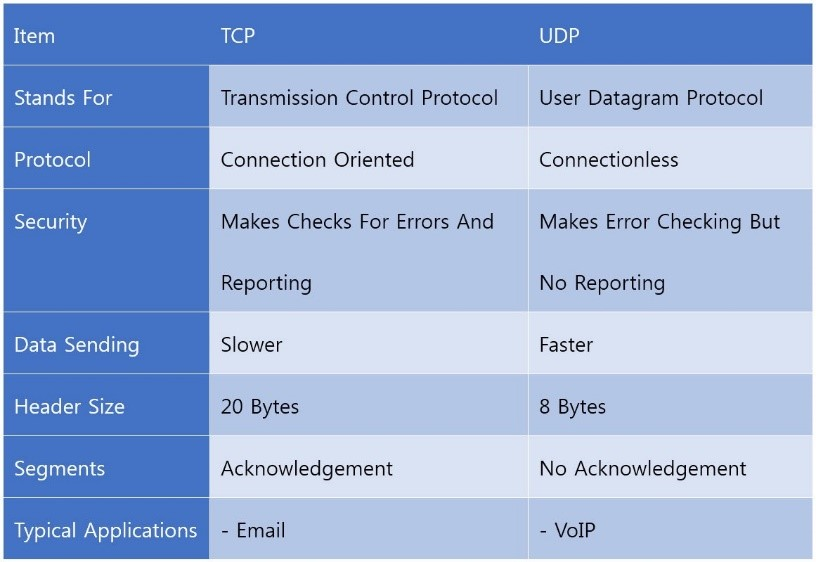
\includegraphics[scale=1.2]{figures/udp_vs_tcp.jpg}
            \caption{TCP vs. UDP. UDP is best for real-time streaming applications, such as this game. \cite{meela_2017}}
            \label{fig:udp_vs_tcp}
        \end{figure}
        The nature of this game necessitates a constant communication channel between a centralized server, Raspberry Pi, and the Unity game engine. A fundamental design choice for the communication was to use the UDP socket protocol over that of TCP. As demonstrated in Figure \ref{fig:udp_vs_tcp}, UDP is preferable for real-time streaming type applications. While there is possibility for UDP datagram loss, this is largely mitigated by the fact that numerous packets are continuously sent. Thus, even if a few are lost, it will not affect game play. The great benefit of UDP is that it is much faster than TCP due to the lack of acknowledgement and continuously open sockets required. UDP is also connection-less meaning it does not require a long-lived connection to function. It will work regardless of the frequency of datagrams that are sent. \par
        The communication network is split up into three main components: 
        \begin{itemize}
            \item Server (Speech and Image Processing)
            \item Raspberry Pi (Sensor Data Acquisition)
            \item Unity Engine (Game Environment)
        \end{itemize} \par
        The server is run in a Ubuntu virtual machine and is written in Python. This is the centralized point where all signals and sensor, speech, and camera data converge. This server opens a UDP socket and binds it to its own IP address. Then, the clients, namely the Unity Engine and the Raspberry Pi, can request and receive responses from the server. It is important to note that the server software is multithreaded as it handles sensor data collection from the Raspberry Pi along with image and speech processing from the server machine itself. \par
        The Raspberry Pi's software is also written in Python. Here, the Pi begins by connecting to the central server. Then, upon receiving a "collect" signal from the server, the Raspberry Pi triggers sensor data collection. Using a UDP socket, linked to the same host IP as the server, the Pi's software sends a continuous stream of position and force datagrams in the form of a JSON package. \par
        Finally, there is the Unity Engine client which also connects to the main server. This client also opens a UDP socket bound to the IP address of the host server. Unity is responsible for sending "collect" and "stop" signals to the server. The server then takes the data from the Raspberry Pi, the processed speech and images from the host machine, and routes them back to Unity as needed by game play situations. All of this information is sent through the network in the form of a JSON package and parsed in Unity through NewtonSoft's asset as referenced in \cite{newtonsoft}.  \par

    \subsection{Testing}
        \begin{figure}[ht]
            \centering
            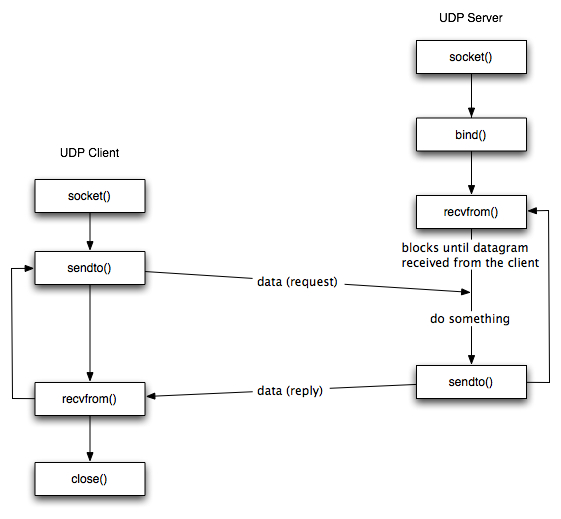
\includegraphics[scale=0.6]{figures/udp_structure.jpg}
            \caption{UDP Socket Programming Structure. \cite{campbell_2012}}
            \label{fig:udp_structure}
        \end{figure}
        The verification of the wireless communication was multifaceted. After following understanding the UDP socket structure as shown in Figure \ref{fig:udp_structure} and reading numerous StackOverflow articles, we developed a simplistic Python server to send and receive strings over sockets. The server was bound to its Wi-Fi IP address assigned by the network. For the purposes of this game, the networks utilized were "eduroam" on the UCLA campus "UCLA-WEB". Additionally, the server sockets were tied to UDP ports 10000 and 10002, which were also opened on the firewall of the host machine. Additionally, since the Raspberry Pi was a client despite needing to respond to requests from the server, we bound port 10000 on the Pi's software as well. \par
        Using a software called PacketSender, we periodically sent UDP packets over the network to the aforementioned ports. The Python server was able to receive these datagrams and print out the string values onto the console. \par
        Upon configuring sockets on the server, Raspberry Pi program, and Unity client, we added more functionality to the server. First, we created separate threads to handle sensor data collection, Unity signal receipt and data sending, speech processing, and camera processing. The server instantiated event objects to trigger and stop data collection from the Raspberry pi on the receipt of collect and stop signals, respectively. Additionally, the server temporarily stores the clients' IP addresses to send responses to any signals. \par
        We verified that the sensor data passed successfully from the Raspberry Pi to the server with print statements and data logs. Similarly, we made sure that the Unity trigger data-grams were sent over the socket to the server and the event objects changed state properly. A large portion of this testing was completed with the use of print statements to facilitate debugging. \par
    \subsection{Progress}
        As of this writing, the wireless communication portion of this game is completely functioning and can handle all situations of game play. The central Python server is able to accept requests from the Unity game engine. Then, the server sends a request for sensor data from the Raspberry Pi and sends this received data, along with the speech and camera information, back to Unity in the form of a JSON package. All of the information passed over Wi-Fi is robust and the entire communication network is modular allowing for easy additions and debugging. Furthermore, the structure of the communication network, which heavily incorporates threading, allows for its successful functioning even with numerous clients. Additionally, even if there is no speech, camera, or sensor data provided, the game will not crash and can easily resume once all functionality is restored. \par
    \subsection{Difficulties Encountered}
        The development of the wireless communication system necessary for this game involved a few challenges that we were able to overcome. \par
        First of all, it was difficult to even find resources to understand UDP socket programming. As a majority of socket work is geared towards TCP and its use in applications that require a continuous connection, it was difficult understanding the use of a connection-less protocol, such as UDP. Upon finding the resources given in \cite{moon_2012}, \cite{karelz}, \cite{raspberry_pi_stack_exchange}, \cite{stack_overflow}, and \cite{karelz_2}, we were able to begin developing the server and the clients using the techniques required for UDP programming. \par
        Along with the difficulties in finding adequate UDP resources, the nature of the Raspberry's Pi software required some intricate tuning of our communication system. The Python server typically sends a "collect" signal to the Raspberry Pi and expects the sensor data in response. This request/response structure is typically implemented on the server; however, the Raspberry Pi is a client. The nature of UDP communication is that one end of the system is a server and the other is the client. The server end is bound to a port and IP address. In our configuration, the IP address on the Python server was bound. However, the Raspberry Pi was performing all of the request/response actions despite being the client. Throughout testing, we found that the Pi's socket would timeout and the Python server would not be able to send it any more requests. Thus, we decided to bind both the server's and the Pi's IP addresses effectively making both ends a "server". This resolved the timeout issue and allows the program to run even if there are long pauses in the game. \par
        Another issue involved in our socket implementation is the fact that we must define the host IP address in the server itself and the two clients. Due the limitations on UCLA's Wi-Fi networks, we were unable to define static IP addresses on the devices, resulting in the need to manually hard code the server's IP address on each run. To circumvent this, we wrote a Python script on the server to automatically get the IP address on each run and establish the socket with this address. However, this does not resolve the necessity of writing the IP address on the client machines. This is still a problem we are working to address. \par
    \subsection{Future Additions}
        The wireless communication network for the game is largely complete, but there are still a few additions that can be made in future iterations of the game. \par
        First of all, as discussed in the Difficulties Encountered section, there is a need to manually program the server's IP address in the client programs. We can attach the host server to a Internet-wide domain name. This name will be static and will alleviate the need to write the IP address in the client software for each run of the game. However, if this is done, only one machine will be able to act as a server limiting the degree of flexibility. \par
        Along with assigning a constant domain, the network can be modified to accommodate more devices during game play. For example, it may be necessary to add one more camera or an extra microphone. To allow for this, we will need to add more sockets and potentially bind more ports to the server. The modular development of the network as a whole allows for these additions to be made quite easily.
\section{Unity Game}
    \subsection{Design}
    The design of our first-person shooter game was split into four stages within our tutorial level. Each stage was designed to measure a skill or combination of skills, and respond to the player's skill level by spawning zombies in particular locations.
    
    \par The first and second stages were designed to isolate the player's skills in depth and aim. The first stage aims at measuring the player's depth in shooting. Three spawn locations were used with varying distances in front of the player. The first zombie is spawned near the player and the player has unlimited shots to destroy the first zombie. Once the zombie is destroyed, a zombie at a further distance is spawned. The player is given five shots to destroy this zombie. If the player fails, the current zombie is destroyed and the previous zombie is spawned. If the player succeeds, a zombie at our furthest location is spawned. Again, for the third zombie, the player has five shots to destroy the zombie, and goes back to the previous part upon failure. Destroying the third zombie allows the player to move on to the second stage. The game logic for the second stage is identical to that of the first stage; however, the second stage aims at measuring the player's horizontal aim, so zombies are spawned at varying horizontal locations.
    
    \par The third and fourth stages were developed to measure the combination of depth and aim by spawning the zombies at varying horizontal locations, but allowing the zombies to move towards the player. The game logic for the third stage follows that of the first and second stages where a tutorial controller is responsible for responding to the player's skill by spawning zombies in locations to match the player's skill level. On the other hand, in the fourth stage, the spawn location of the zombie is determined by a second player. The second player can analyze the shooting skill's of the player and select between four locations to spawn the zombie with the intention of improving the player's weaknesses.
    
    \par In addition, C\# scripts were created and attached to the player, zombie, HUDCanvas, EnemyManager, and TutorialController game objects to give them the desired behavior. The player was given the ability to take damage if a zombie enters the volume of its sphere collider. Further, the player was given the ability to shoot an arrow and change its rotation based on input from our server. The zombie was given the abilities to attack a player, take damage from an arrow within its sphere collider, and move towards the player. The HUDCanvas was responsible for keeping track of and displaying the current stage, the number of zombies left in the tutorial level, the player's health, and the start and end screens. The EnemyManager was designed to spawn the zombies and record references to each of the currently spawned zombies. Lastly, the TutorialController implemented a state machine to handle the state transitions between our four stages. 
    
    \subsection{Testing}
    To verify the functionality of the tutorial level, the IMU was used to determine the rotation of the player and the mouse button was used to fire the arrow. The first three stages were tested by performing the following sequence of test cases. These test cases allowed us to verify that the player can appropriately progress through the stage with our intended game logic. 
    
    \begin{enumerate}
        \item Miss the zombie more than 10 times
        \item Destroy the zombie with two body hits
        \item Miss the zombie five times
        \item Destroy the zombie with head shot
        \item Destroy the zombie with two body hits
        \item Miss the zombie five times
        \item Destroy the zombie with head shot
        \item Destroy the zombie with two body hits
    \end{enumerate}
    
    \par In order to test the game logic of the fourth stage, the keys 'u', 'i', 'j', and 'k' were used to spawn zombies in one of the four spawn points. Two main requirements were verified for the fourth stage. If a zombie reaches the player and eats him, the game ended. If the player successfully destroys five zombies, the game ended. 
    

    \subsection{Progress}
    As for the tutorial level described in the Design section, each stage was implemented with its intended functionality. Furthermore, the functionality of the five main game objects described was implemented successfully. Images of game play are shown in Figures
    \ref{fig:Stage1} and \ref{fig:Stage4}. 
    
    \begin{figure}
            \centering
            \includegraphics[scale=0.3]{figures/Stage1.png}
            \caption{Set-up of the second zombie in stage 1.}
            \label{fig:Stage1}
        \end{figure}
        
        \begin{figure}
            \centering
            \includegraphics[scale=0.3]{figures/Stage4.png}
            \caption{Set-up of multiple zombies in stage 4.}
            \label{fig:Stage4}
        \end{figure}
    
    \subsection{Difficulties Encountered}
    One of the difficulties in implementing the tutorial level for the ZombieArcher game was the learning curve associated with Unity. Initially, it took various tutorials found on the web to learn how to set up the programming environment, how Unity scripts model the behavior of game objects, and what libraries Unity offers. Specifically, many tutorials from the Unity website were used to help write code for the first-person shooter game, and were targeted towards our game. \cite{unity_tut}
    
    \par A more important difficulty we encountered was deciding on how to organize our tutorial level to measure the player's skills. Although the purpose of our first two stages was to isolate specific skills of the player, the player's lack of the non-measured skill can prevent the player from completing a stage. For instance, in the stage where the depth of the player is tested, the player can miss the zombie by shooting off to the side and our game would deem the player's skill in depth as inadequate when it is clear that the player needs to improve his horizontal aim. More work will be done in the following quarter to address this problem and properly isolate the player's skills. 
    
    \subsection{Future Additions}
       For the following quarter, we plan on improving our methods for data collection within Unity. Currently, our tutorial stage simply counts the number of misses by the player, and respawns the previous zombie if the player misses five times. It does not keep track of which stage the player was missing in or store the data for future levels. Instead, we plan on storing this data and responding to the player's deficits by creating a decision tree to decide where the best location is to spawn the zombie, with the objective of exploiting the player's weaknesses. In addition, there is much work to be done to improve the game mechanics in order to provide a more realistic and enjoyable experience including adding zombie animations, improving the shooting mechanics of the arrow, and adding sound effects. 
    
\section{Image Processing}
    \subsection{Design}
    ZombieArcher was designed to detect player movements with the computer's camera. Because of limited time provided and the difficulty with accurate facial recognition, we have required the player to wear a bright pink hat and bright green gloves. This will make it significantly easier for the camera to detect the player. As of this writing, we do not have those materials so we have tested the detection with a blue phone screen instead.\par
    The image processing was implemented in Python using the OpenCV package and was largely based off of the work of \cite{Mordvintsev_2013} and \cite{Sharma}. The program first opened up the camera and analyzed the video frame by frame. From there, each frame was converted to a HSV (Hue Saturation Value) image as it is easier to analyze it with this color scheme than in RGB (Red Green Blue). Then the HSV image was thresholded to create a mask which kept only the color we wanted and made the rest of the frame black. Finally, the mask was bitwise-ANDed with the original image to keep only the color in the frame we wanted and filter out everything else. After the frame had been filtered, a blur was applied to smooth out the image and reduce background noise. This was to stabilize the image, making it easier for the camera to detect the pertinent object and prevent the camera from detecting any extraneous objects or light that might have been in the background. After the blur was applied, the camera found the contours of the image and drew a rectangle around it to track the object. In addition, the coordinates of the contours were tracked to tell the game whether the object was ducking or standing and what quadrant it is in.
    The steps of the image processing are shown at the top of the next page:
    \begin{figure}[h!]
        \centering
        \begin{subfigure}[b]{0.4\linewidth}
            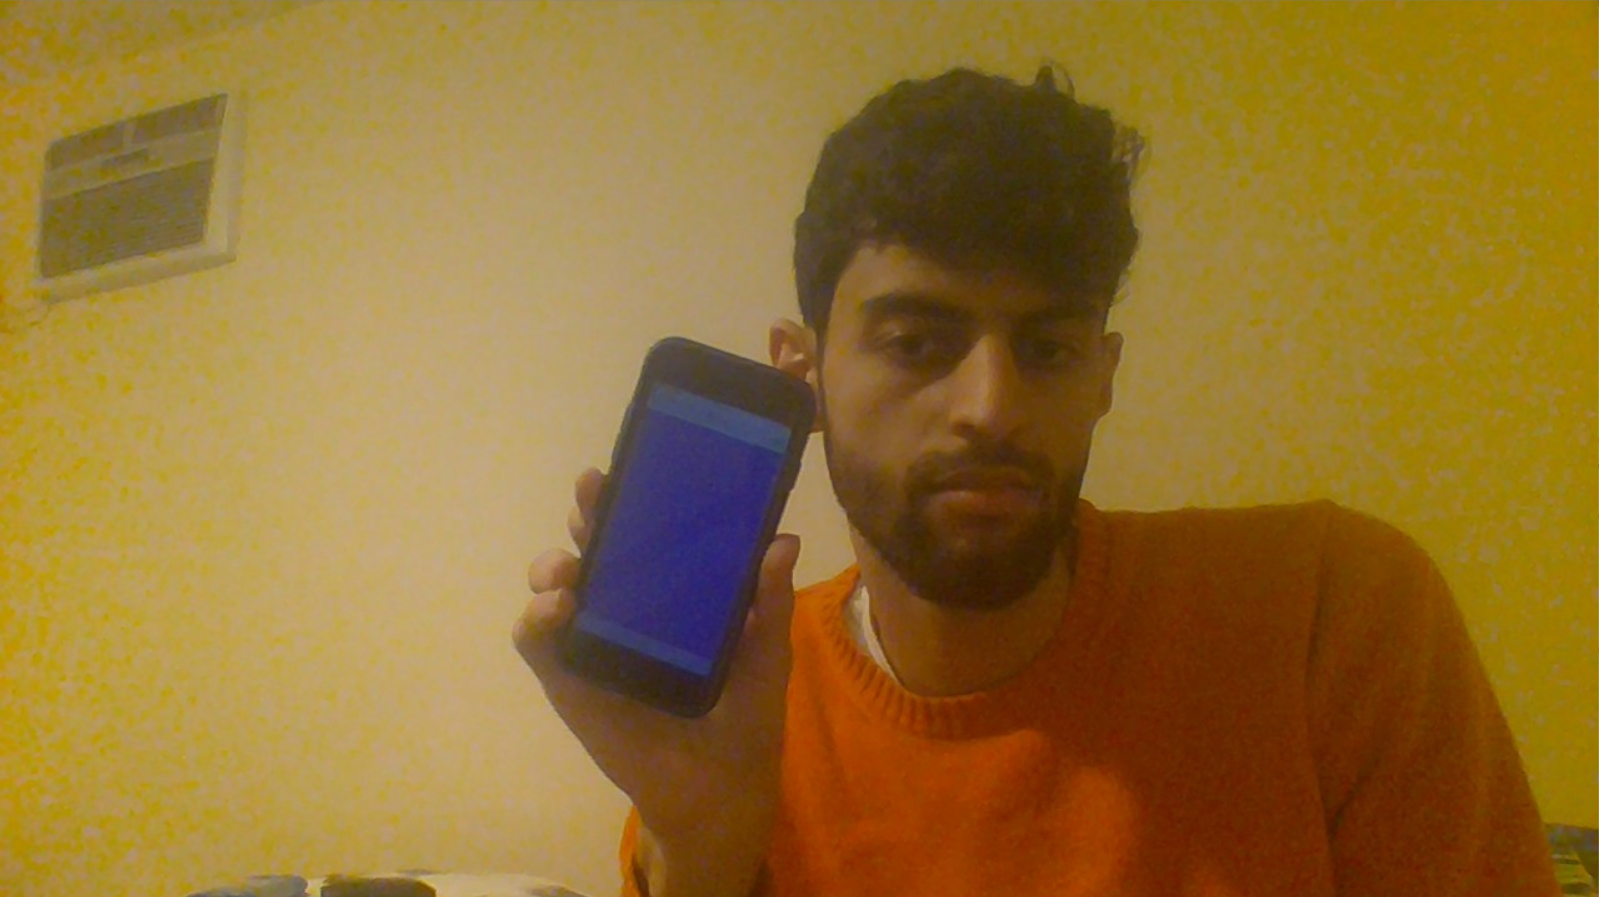
\includegraphics[width=\linewidth]{figures/Capture5.PNG}
            \caption{The original image}
        \end{subfigure}
        \begin{subfigure}[b]{0.4\linewidth}
            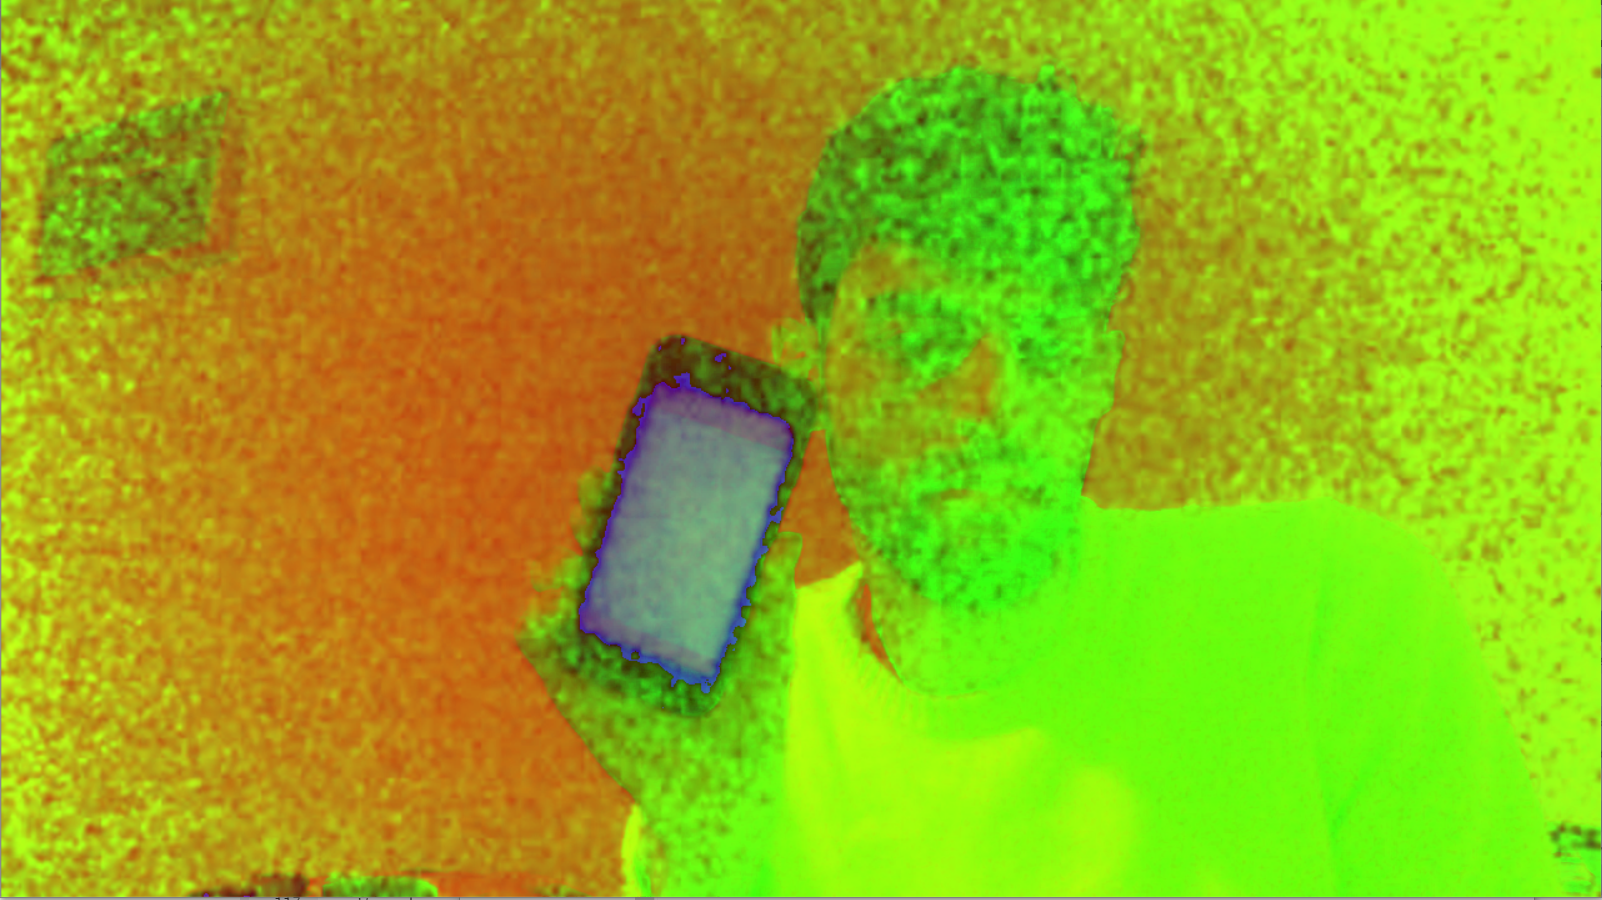
\includegraphics[width=\linewidth]{figures/Capture4.PNG}
            \caption{Image converted to HSV}
        \end{subfigure}
        \begin{subfigure}[b]{0.4\linewidth}
            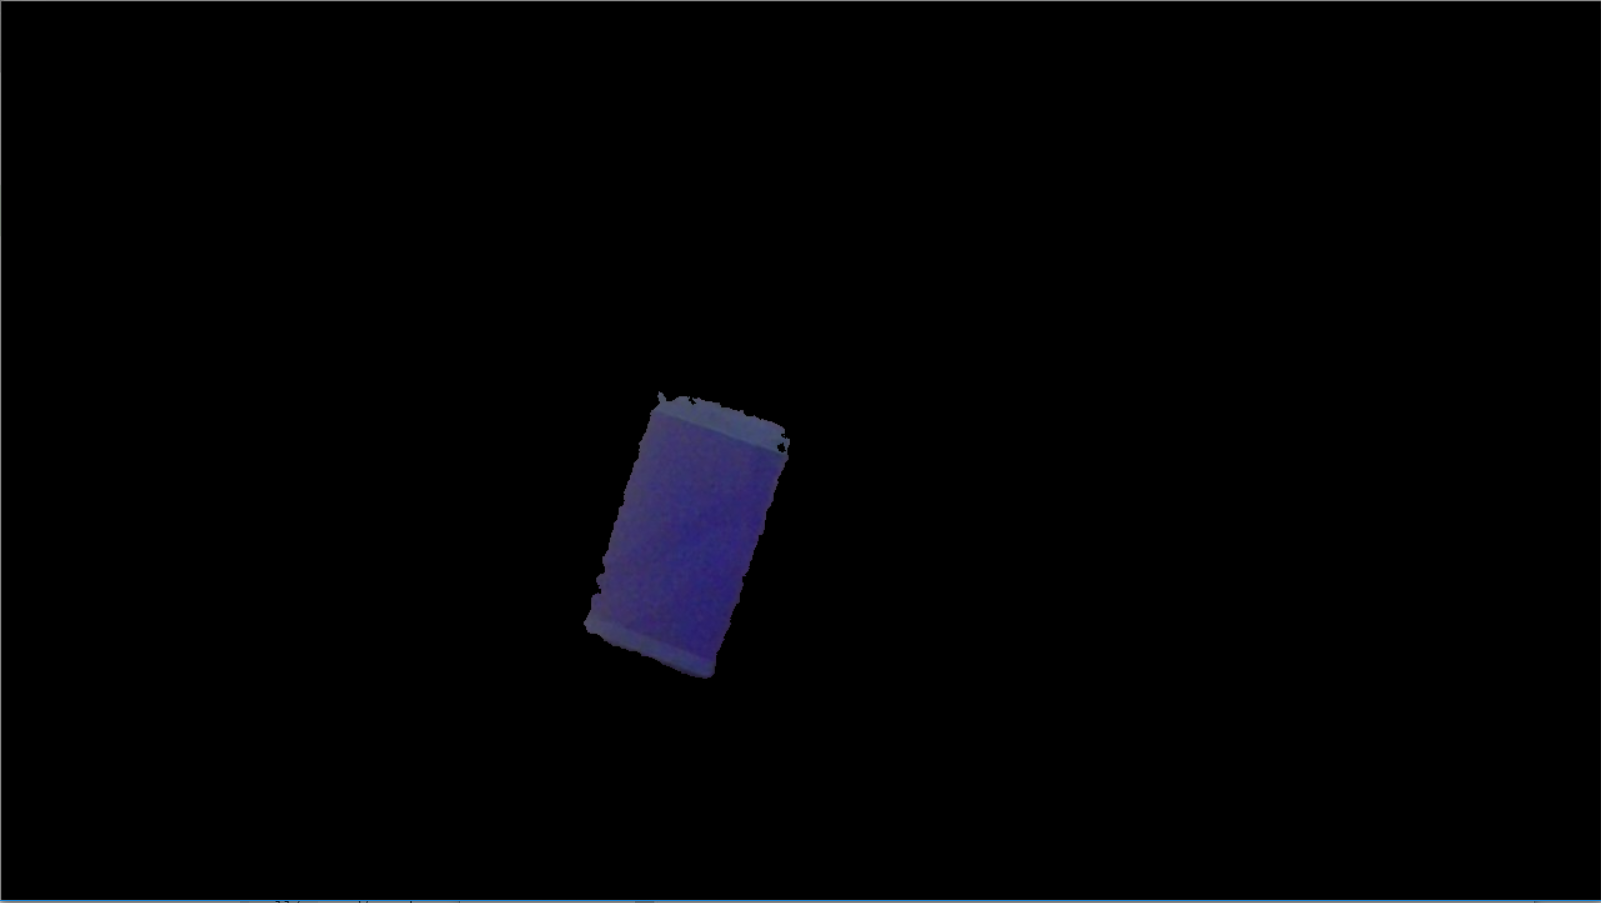
\includegraphics[width=\linewidth]{figures/Capture3.PNG}
            \caption{Threshold mask applied}
        \end{subfigure}
        \begin{subfigure}[b]{0.4\linewidth}
            
\includegraphics[width=\linewidth]{figures/Capture2.PNG}
            \caption{Blurring applied to reduce noise}
        \end{subfigure}
        \begin{subfigure}[b]{0.4\linewidth}
            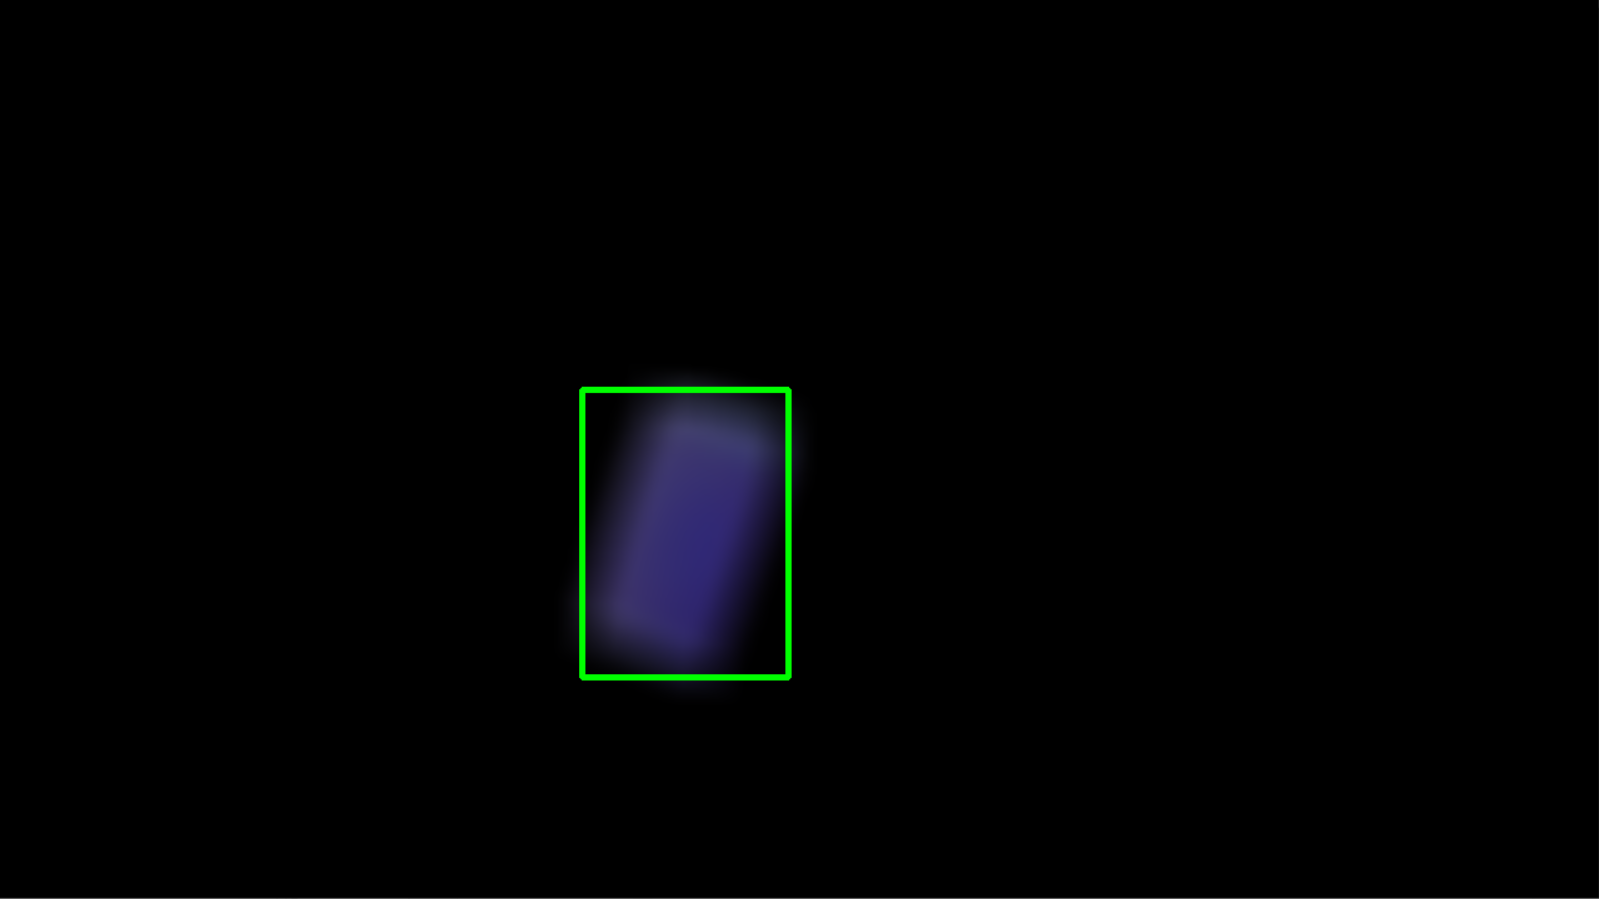
\includegraphics[width=\linewidth]{figures/Capture1.PNG}
            \caption{Bounding rectangles applied}
        \end{subfigure}
        \caption{How an image gets processed to get the desired color}
        \label{fig:Images}
    \end{figure}
    \subsection{Testing}
    The image detection was tested extensively in many environments with different background colors, dust levels, and lighting. We also made sure the camera was able to detect slow and rapid movements.\par 
    We made sure that the camera picked up on the desired color by playing with the range of the threshold values. If we picked a too narrow range, then the camera did not pick up anything but if we picked too wide a range, then the camera picked up too much. Once we had chosen the appropriate range, we tested the camera too see that it had picked up a desirable amount of the color we were looking for. Of course, nothing is perfect and there was always noise that was picked up but we made sure that the noise was minimized. \par
    After choosing the correct range of colors, we tested the camera under different levels of light and in rooms of varying dust levels and background colors. These things affect the camera quality and the color perceived by the camera so we must make sure that these are accounted for. Under the abnormal conditions, the perceived object was obstructed so we compensated for this by blurring the final image in the design to reduce noise and make the object homogeneous in color. \par
    Finally, we tested the robustness of the camera by making the object move rapidly and making sure that the camera still tracked the object and returned its position. Fortunately, the camera detected the object effortlessly and we did not have to make any modifications. Next, we put the object in the lower and upper halves of the screen and made sure that the program returned ducking and standing, respectively. We also put the object in each quadrant of the screen and made sure that the program returned the right quadrant. 
    \subsection{Progress}
    We are mostly done with the image processing part of the project. It is does what we want and performs reliably under different environments. As of this writing, it works with blue but we are most likely going to change that to another color which is a trivial task. Also, if we need to change the blurring level for any reason that is also a trivial task.  
    \subsection{Difficulties Encountered}
    Finding the right environment to work with was definitely the most difficult part. After that, ensuring that the code did what we wanted it to was somewhat of a challenge but not as hard as setting up the environment. \par
    At first, we started coding in Pycharm, which was a complete disaster since it was slow, crashed a lot, and all of the libraries that we needed refused to install. This was very frustrating and made us get off to a slow start. After that we switched to Spyder, which was only marginally better since the libraries actually installed, but it was still slow and bulky. Finally, we switched to writing my code on Notepad++ which was lightweight and easy to use and ran it on command prompt. This set up was easy, lightweight, fast, and everything worked smoothly.\par
    After finally finding the right environment to code in, the next task was to actually write code that did what we wanted. We searched the internet looking for tutorials and documentation that showed us how to use OpenCV's functionality. We progressed slowly, starting off with opening up images and changing their colors. Then we moved on to videos and added more sophisticated filtering techniques. We made sure to do everything incrementally, as the code was initially hard to understand and because bugs kept popping out of nowhere. The last thing we did was integrate the image processing with the game. Despite the hardships and the seemingly impossible bugs, we managed to come up with a program that meets our needs. 
    \subsection{Future Additions}
    In the future, we would use a more sophisticated noise reduction method, as blurring the image ruins the sharpness of the image and does not always completely eliminate the background noise. Also, we would like to see more features implemented in the game. The image processing works fine so there is a lot of opportunity to add more actions in the game. So far we have ducking and standing but we could also add hand signaling and possibly even melee attacks. Either way, we are excited for the future of this game.
    
\section{Speech Processing}
    \subsection{Design}
        ZombieArcher was developed to respond to certain explicit commands issued by the player during game play itself. For the first phase of game development, the primary commands were those send to start and pause the game. \par
        The bulk of the speech processing was completed within the Python server. Using the SpeechProcessing Python wrapper, the server instantiates a microphone object and recognizer object in a separate thread. The thread calls the listen() method and continuously listens for audio commands. Once a player issues a command, the microphone picks it up and stores the audio. This audio is then passed to the recognizer and, using Google's speech-to-text API, the recognizer returns a string representing the content of the audio. A control statement compares the string to a pre-defined list of commands and, if a command matches,it is written to a variable. This variable is then sent over the UDP socket to Unity, where the game dynamically responds by either starting or pausing. \par
        When the recognizer object is created, the Google API is defined as the speech recognition service. We chose Google over IBM, Bing, and PocketSphinx for a variety of reasons. First of all, Google's API was the most accurate and its documentation was easy to follow. Additionally, Google's bank of audio data is large enough to accurately discern distinct commands issued. Additionally, the microphone object was instantiated to use the default microphone, which was part of the integrated camera on our host machine. However, the microphone was also tested with that on an external web-cam and we could easily define which microphone to use. \par
    \subsection{Testing}
        \begin{figure}[ht]
            \centering
            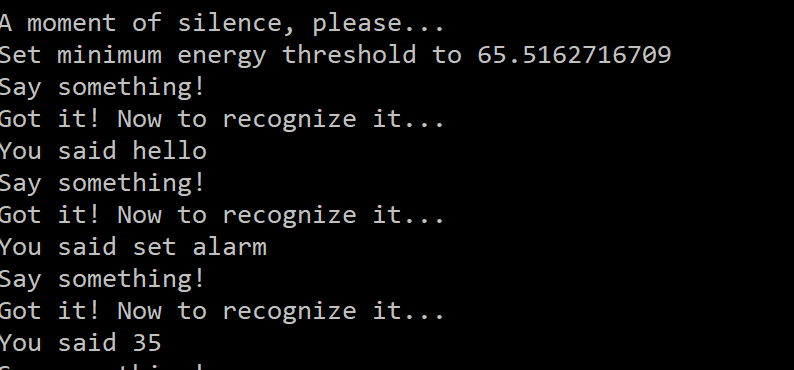
\includegraphics[scale=1.2]{figures/speech_processing_testing.PNG}
            \caption{Successful speech recognition with the Google API and Python SpeechProcessing wrapper.}
            \label{fig:speech_testing}
        \end{figure}
        After understanding the functioning of the SpeechProcessing library as referenced in \cite{amos_2018} and \cite{uberi_2018}, we performed numerous unit tests before building the program best suited for this game. Based on the use cases given in the library's documentation, we decided to implement a structure in which the microphone constantly listens for commands and, upon any input, recognizes the audio. If the recognized audio matches any of the defined commands, variables would be modified and sent to the server. \par
        As a first test, we used the listening code provided in the library's GitHub. Then, we tested all of the potential speech recognition API's, which include CMU Sphinx, Google Speech Recognition, Google Cloud Speech, Wit.ai, Microsoft Bing Speech, Houndify, and IBM Speech to Text. After researching all of these potential API's, we decided on Google Speech Recognition as it was one of the most accurate and efficient recognition engines. \par
        Furthermore, we practiced our commands, primarily "play" and "pause", with the Google API numerous times and collected log data depicting the accuracy of the recognition system. One we were confident that Google's API would be able to recognize the commands, we created a public variable that would hold the state of the command and be passed through the server to the Unity client. Through this variable, we can use speech to control the state of the game. \par
    \subsection{Progress}
        Currently, we have implemented speech recognition in this project to a substantial level. The server spawns a thread that constantly runs and listens for audio input. After input is detected, the program passes the audio to the recognizer and the Google Speech API returns a string with the closest match. Once we have a match to one of the commands, the software modifies the appropriate variable, which is then sent to Unity and utilized by the game. As of now, there are two commands to interact with the game, namely "play" and "pause". In the coming iterations of the game, these commands will be further refined and more features will be added. 
    \subsection{Difficulties Encountered}
        While developing the speech processing infrastructure necessary for our game, we encountered a few roadblocks. However, after substantial debugging and research, we were able to solve all of our issues, which are enumerated below. \par
        Before developing anything with regards to speech processing, we ran into issues with Python and microphone input on the host machine. For all other development, we used the Ubuntu WSL feature on a Windows 10 machine. However, upon starting speech recognition work, we quickly found that Microsoft's WSL software does not support the use of external hardware. Thus, we decided to create a virtual machine running the Ubuntu Server operating system in Oracle VirtualBox. After some tweaking and research, we were able to pass the microphone from the host machine to this virtual machine and continue with development. \par
        After setting up the environment, we proceeded to install the SpeechRecognition library inside Python, but we ran into another roadblock when trying to read input from the microphone. It turns out that Ubuntu machines need a few more drivers, such as AlsaMixer and PulseAudio, to work with audio input devices. After installing these and increasing the sensitivity the microphone, we were able to get input and begin development. \par
        Despite these minor impediments, audio processing was largely fruitful due to the clear Google API and Python SpeechRecognition documentation. However, we have noticed a high latency with Google's API, which is not a major impediment to our gameplay as the commands are largely time invariant for now. Thus, we will most likely be moving away from Google Speech to Text as the game's functionality increases.
    \subsection{Future Additions}
        Although our game implements and utilizes speech recognition and processing, there are many additions that can be made to enhance the game. \par
        First of all, we have not yet tested the speech recognition functionality in a loud environment. After doing this, we may find that our current implementation may not be successful for in all conditions. Thus, we may need to do some calibration at the start of the game to establish a minimum ambient sound threshold to prevent the microphone from picking up any noise. \par
        Additionally, we hope to look into neural network based hotword detection algorithms and libraries, such as Porcupine \cite{picovoice_2018}. This will allow us to reduce our dependency on Google's API, its stringent audio file limitations, and its high latency. Furthermore, we should be able to obtain excellent accuracy and fast recognition by training our models with large enough sets of data. \par
        Along with ambient noise adjustment and offline detection systems, future versions of the game can incorporate different voice commands. The method of recognizing key words and phrases through the Google Speech to Text API is straightforward enough that only minor changes will be required to include varied instructions. Furthermore, it is not too difficult to send the results of these commands to clients within the aforementioned JSON package. \par

\section{Integration}
    \begin{figure}
        \centering
        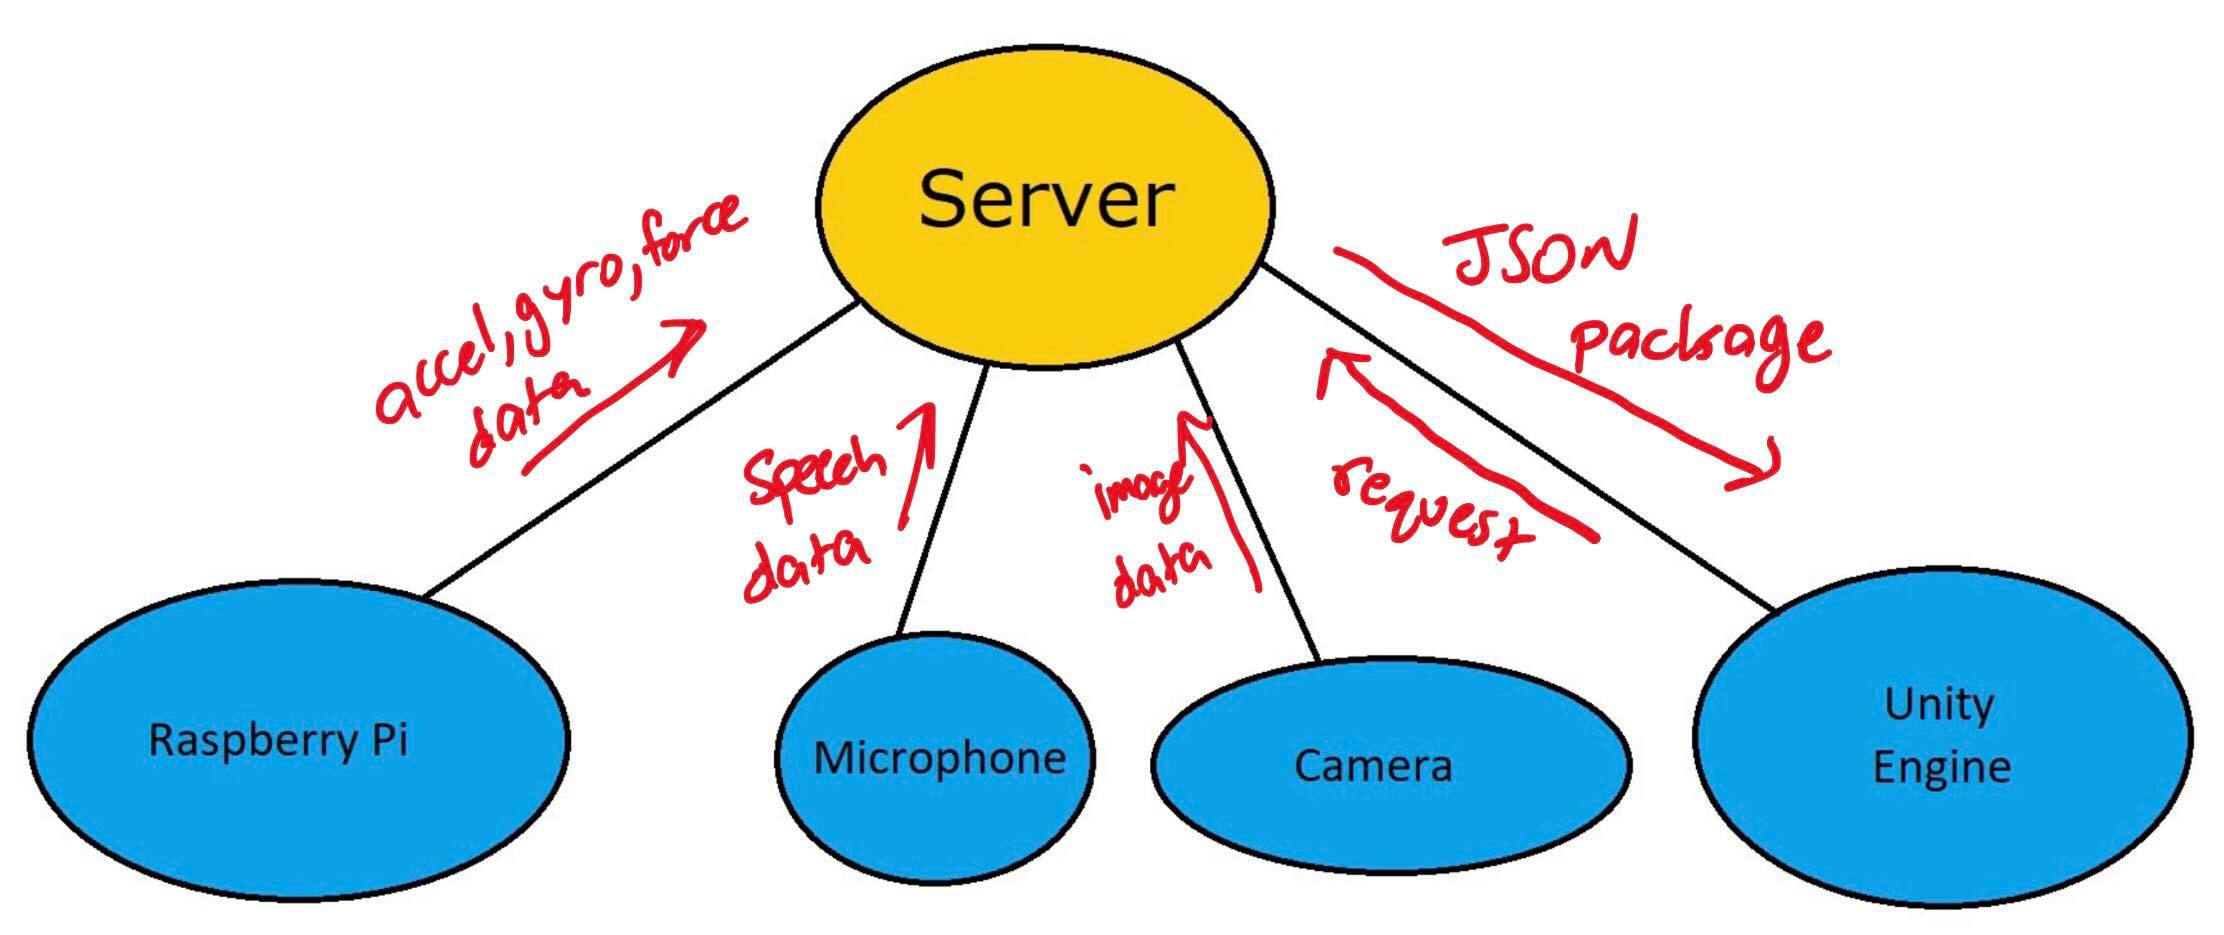
\includegraphics[scale=0.2]{figures/flow_chart.jpg}
        \caption{Process Flow Diagram. Depicts the movement of data throughout the game-play process.}
        \label{fig:flow_chart}
    \end{figure}
    The flow chart given in Figure \ref{fig:flow_chart} shows the movement of data throughout the varied components of our game. First, the Unity engine sends a request to the server for the data. Then, after receiving the request, the server requests the clients for data. The Raspberry Pi is responsible for sending the force, acceleration, and gyroscope data. Also, the microphone and camera send the speech and image data, respectively. Once the server collects all of this data, its packaged into a JSON object and sent to Unity where it is parsed and used within the game. \par
    An important design choice for our communication system is its modular nature. This allows for more clients to be easily incorporated in the future. As we hope to develop a true multi-player mode in future iterations of the game, it may be necessary to add a second Raspberry Pi controller. Additionally, we may need to add a second camera to alleviate the gyro drift. All of these additions should be quite straightforward with the network we have developed.
    \subsection{Testing}
    In order to test the integration of the various components, we verified that the data sent to the server was correctly packaged into a JSON object by displaying the object's fields in a console. While the console was displaying the data, stimulus was provided to each of our sensors and we examined whether the data displayed corresponds to the data expected as a result of the stimulus. If the data showed on the console for a particular server was not displaying the expected data, we tested the sensor in isolation. After it was verified that the server was properly receiving and packaging the data, the process was repeated for the Unity client. Data was displayed on Unity's console and was used as stimuli to the game logic to verify the connection between the Unity client and server. 
    \subsection{Challenges}
    One of the challenges of integrating the different features of our game was that one person had the Unity game functioning on his laptop and another person had the necessary tools to run the server on his laptop. If, for instance, the person performing image processing wanted to test how his code affects the gameplay, these two persons needed to be around, giving the person performing image processing less opportunities to test his code with the game. Although this did not hold us back significantly as most of our work this quarter was able to be performed independently, we anticipate this to be a problem for the following quarter. As a result, we plan on spending time early on next quarter on project management, where we can show each other how to set up the Unity game and server. Then, each person in our group will have more opportunities to test their code before we spend time integrating components together.
    
\section{Future Work}
    In the next version of the game, we hope to add many new features. Particularly, we would like to focus on the machine and iterative learning aspect of the game. As a player progresses through the tutorial and subsequent levels, the game should collect player statistics, such as the number of zombies killed, hit percentage, and average time taken to kill a zombie. Using this information, we can spawn zombies that exploit the player's weaknesses. This will further test and strengthen each player's cognitive ability in a unique manner. Additionally, the zombies themselves can be made "smarter" so to speak. They may now be able to dodge certain arrows and move in randomized patterns. \par
    Along with this iterative learning, we hope to implement enhanced sensor fusion. Mainly, we want to reduce gyroscopic drift in our tilt angles as much as possible. To do this, it may be necessary to add a second camera and possibly, another IMU. \par
    Lastly, we hope to implement a proper multiplayer mode. This can either be adversarial or supportive. Perhaps, two players can compete to kill more zombies. On the other hand, we can allow players to collaborate in an effort to kill zombies more successfully. This mode will surely require more sensors and clients to be incorporated to our network.

%%%% Adding the bibliography from external file
\nocite{*}
\bibliographystyle{IEEEtran} % We choose the "IEEEtran" reference style
\bibliography{references} % Entries are in the "references.bib" file

\end{document}
